\chapter{Background}
\label{ch:background}

\graphicspath{ {./body/media/} }


In this chapter, we develop the theoretical intuition for the basic approaches used in Deep Learning and Natural Language Processing. The goal is a concrete understanding of the foundation upon which our work is built.

\section{Artificial Neural Networks}
\label{sec:anns}

Scientists have long studied the human brain and sustained large interest in its versatility in learning. A substantial amount of research has gone into figuring out how the human brain can achieve such a high level of versatility. This has provided some useful insights into how the human brain works, however, we are still pretty far from fully understanding how a brain functions. In the field of artificial intelligence (AI), researchers have been able to provide some effective solutions to many problems by translating the observations and conclusions of biological research of the brain.

The human brain is part of the nervous system, which consists of nerve cells (or neurons). In fact, the brain is a huge interconnected network of neurons. The robustness of this huge network makes it virtually impossible to model it with the currently available technologies. The aim of computer scientists is, however, different. The goal is to rather simulate this thinking or learning process without the need to fully model or understand it.

An Artificial Neural Network (ANN) \citep{mcculloch1943logical} is a computing system designed to mimic the human brain. An ANN is a network of interconnected components or units called perceptrons. The connections between these units are modeled as numerical real numbers -- weights. A positive weight indicates an excitatory connection, while a negative one indicates an inhibitory connection. These weights adjust according to the learning procedure and modify the input to produce an output. Finally, an activation function is applied to this output to control its magnitude.

The perceptron \citep{rosenblatt1958perceptron} is an algorithm for binary classification, where it performs a weighted sum of the (input) feature vector elements to decide whether or not an input belongs to some class (as shown in \cref{fig:perceptron}). Concretely, the perceptron takes as input a real-valued vector $\mathbf{x} = (x_1, x_2, \ldots, x_n)^T$ and computes the following function:
\[ \hat y = \sigma (\mathbf{w} \cdot \mathbf{x} + b) = \sigma (\sum_{i = 1}^{n} w_i \cdot x_i + b) \]

where $\mathbf{w}$ is the weight vector, and $b$ is a bias term used to shift the decision boundary and is independent of the inputs. $\sigma = \dfrac{1}{1 + \exp(-x)}$ is the sigmoid activation function that squishes the output between 0 and 1 to create a probability output.

\begin{figure}[ht]
\centering
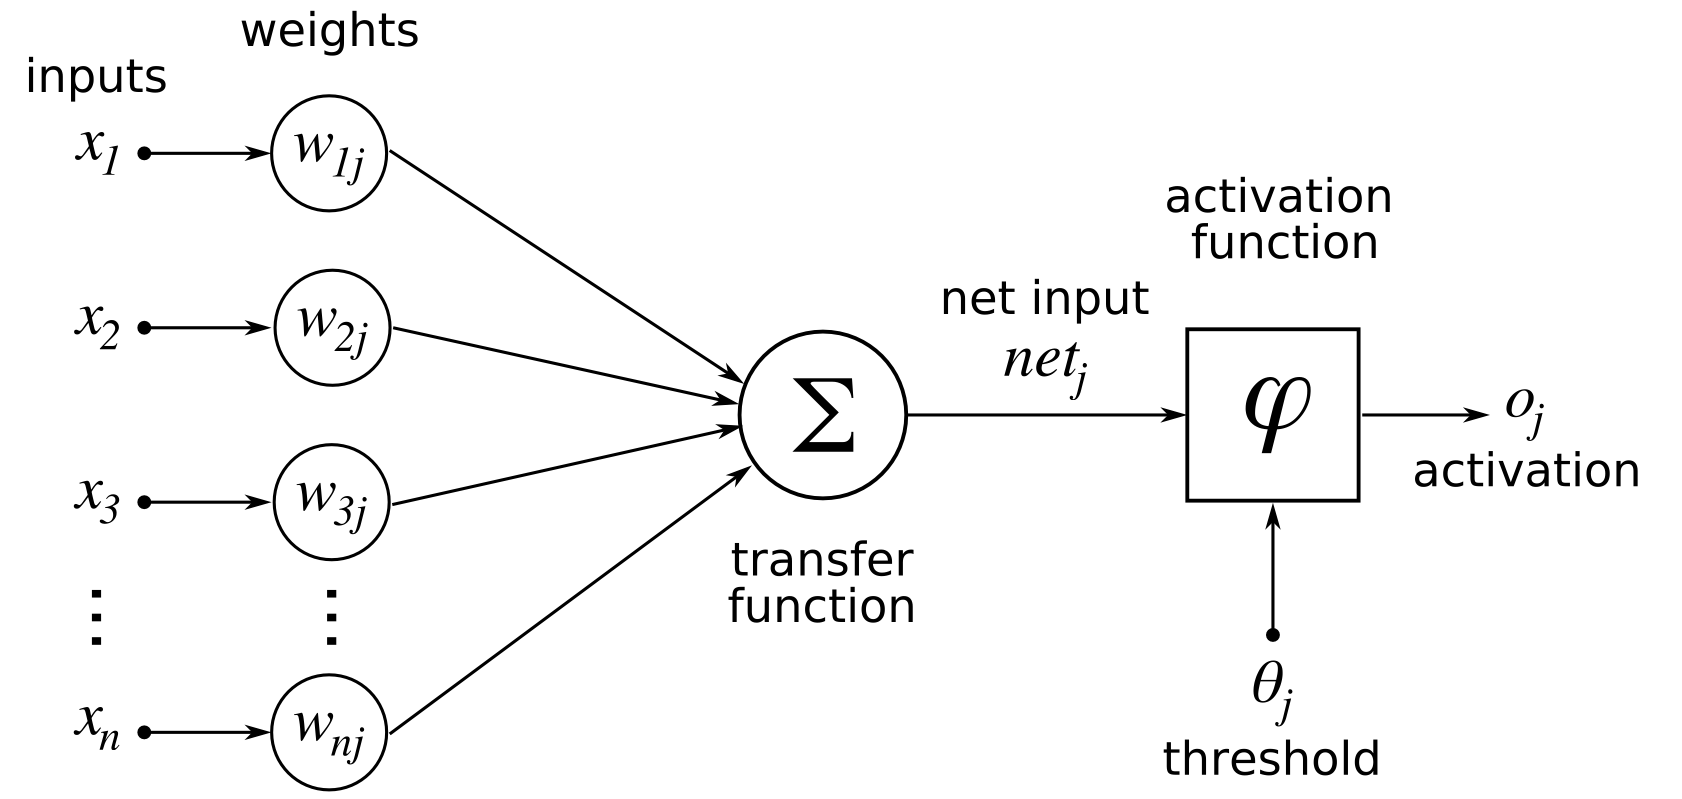
\includegraphics[scale=0.2]{ArtificialNeuronModel_english}
\caption{The Artificial Neuron (Perceptron) \protect\footnotemark}
\label{fig:perceptron}
\end{figure}
\footnotetext{\url{https://en.wikipedia.org/wiki/Talk:Artificial_neuron}}

To learn more powerful models that can perform more complex tasks, the perceptron units are grouped in layers, and these layers are stacked to build deep neural networks (also called multilayer perceptron -- MLP). Traditionally, there are three types of layers; input layers which receive the instances of the data, output layers which produce the results of the network's computations, and hidden layers which lie in between input and output layers and are responsible for computing hidden representations of the previous layers' outputs. The deeper (i.e. latter in the stack) the hidden layer, the more complex representations it is supposed to learn. A network is considered deep when it has two or more hidden layers. In this context, we are more interested in dense layers or fully connected layers, that is layers that have connections between all the neurons.

A deep neural network -- shown in \cref{fig:deep_network} -- is a machine learning (ML) algorithm that uses a hierarchical sequence of $n$ parametric functions to model the input $\mathbf{x}$. Each function $f_i$ ($i \in \{1, 2, \ldots, n\}$)  is modeled as a layer of neurons that apply the perceptron algorithm on the previous layer's output. As a generalization of the perceptron, each layer $l_i$ is parameterized by a weight matrix $\mathbf{W}_i$ applied on the immediate input of $l_i$. Formally, a deep neural network computes the following function:
\[ \hat y = f_n( \mathbf{W}_n, f_{n-1}( \mathbf{W}_{n-1}, \ldots, f_1 (\mathbf{W}_1, \mathbf{x}) ) ) \]

\begin{figure}[ht]
\centering
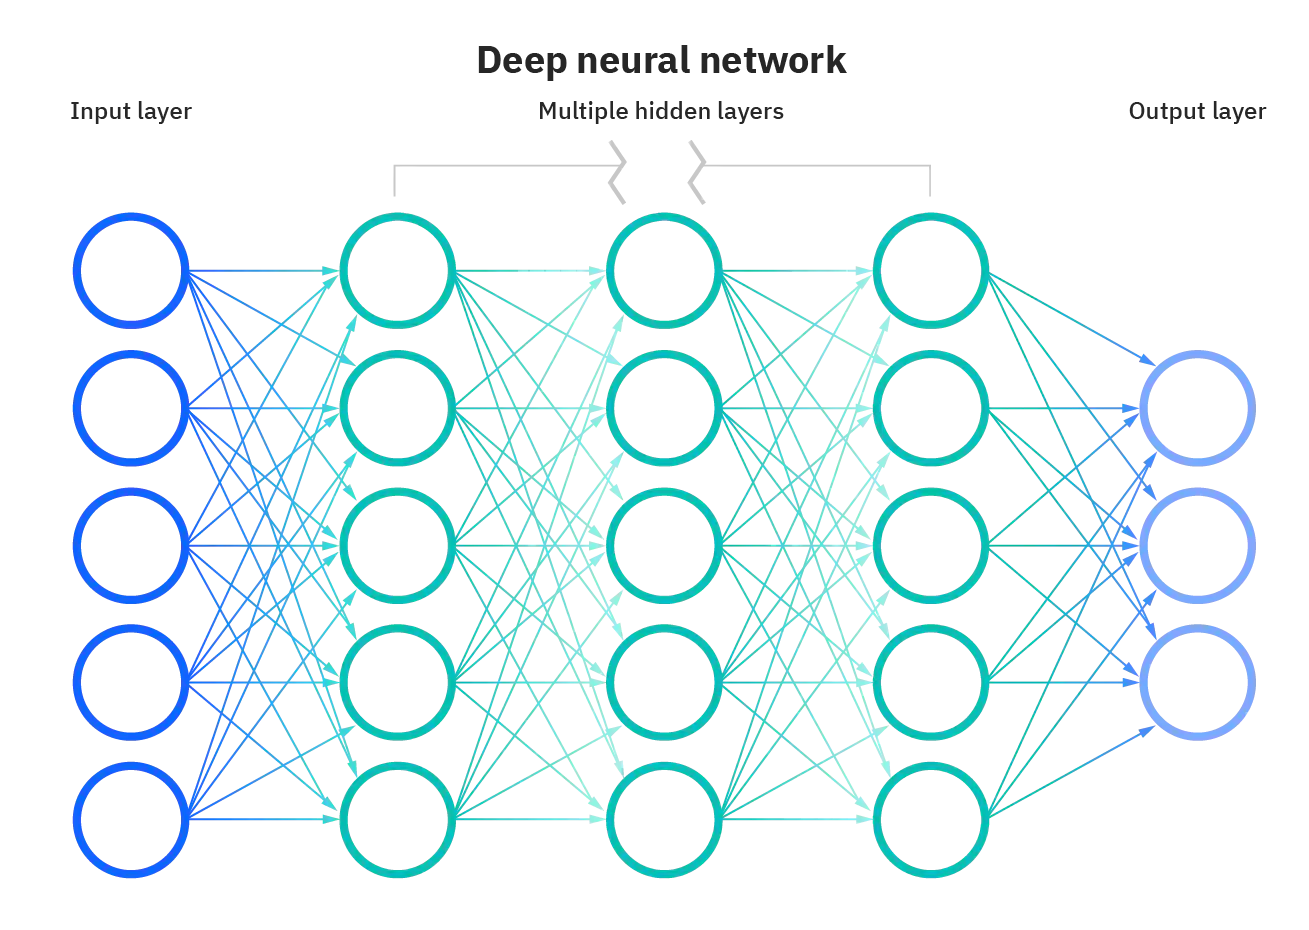
\includegraphics[scale=0.2]{DeepNeuralNetwork}
\caption{Deep Neural Network \protect\footnotemark}
\label{fig:deep_network}
\end{figure}
\footnotetext{\url{https://www.ibm.com/cloud/learn/neural-networks}}

The ability to learn is the key concept of neural networks. During the training phase, the network tries to find the optimal parameters $\mathbf{W}_i, \; i \in \{1, 2, \ldots, n\}$ for solving a given task. Before the training process, the parameters are initialized to some random values which are tuned later according to some error measure. Learning is then carried through an iterative process where we feed the data to the network (called forward pass), analyze the outputs, and repeatedly tune the network for better performance. The outputs are analyzed through a cost function  $J(\hat y, y)$ that measures the error between the prediction $\hat y$ and the true label $y$ for the associated input vector $\mathbf{x}$. The weight tuning procedure is, formally, finding the set of optimal parameters that minimize the cost function $J$. This is done by using the backpropagation algorithm (BP), which computes the gradients of the cost function with respect to the network's parameters ($\nabla_{\mathbf{w}} J$), and then propagates them back from the output layer to the input layer to determine the weight update value according to the formula:
\[ \mathbf{w}^{t+1} \leftarrow  \mathbf{w}^{t} - \eta \ \nabla_{\mathbf{w}} J  \]

where $\eta$ -- the learning rate, defines the amount of weight adjustment. In the evaluation phase, the network's parameters are frozen and the predictions are obtained through a forward pass.

Activation functions are functions that map the input space to a different output space, and they control the information flow between layers in an MLP. These functions have to be continuously differentiable to allow gradients to flow in the backward pass of BP.

According to the universal approximation theorem \citep{csaji2001approximation}, neural networks are universal function approximators. That is, an arbitrary continuous function can be approximated using an MLP with one hidden layer and an arbitrary number of neurons in that layer. For this theorem to hold, the activation functions need also be non-linear, so that the output is non-linearly dependent on the input.

The most commonly used activation functions are \texttt{sigmoid}, \texttt{softmax}, \texttt{tanh} and \texttt{relu} among others.


% =================================================================================================

\section{Word Embeddings}
\label{sec:embeddings}

Deep neural networks deal with numbers and not symbols. In general, an embedding is a representation of a symbol (e.g., word, character, or sentence) in a low-dimensional space of continuous-valued vectors. In natural language, words are not discrete isolated symbols, rather they are correlated with each other. Projecting these continuous-valued vectors into euclidean space visualizes the relationships between words. Depending on the task, we can learn the similarity (distance in Euclidean space) between different word representations.

Word2Vec \citep{mikolov2013distributed} aims to learn a universal embedding matrix $\mathbf{E} \in \mathbb{R}^{V \times d}$ where $V$ is the vocabulary size and $d$ is the dimension of the vector representation. Each row $\mathbf{e}_i$ of $\mathbf{E}$ corresponds to the unique embedding of token $i$ in the vocabulary $V$. This can be learned through one of two methods: continuous bag-of-words (CBOW) or skip-gram. In CBOW, the model predicts the current word from a window of adjacent context words, while skip-gram is the reverse.

Traditional word embeddings suffer from their inability to discriminate different meanings of the same words under different contexts \citep{camacho2018word}. For instance, the word \textit{bank} can refer to two different meanings depending on the context: a financial institution or a sloping land near a body of water. Such words are said to be ambiguous and each meaning is called a word sense.

Sense embeddings attempt to model individual word senses into independent vector representations. This technique mainly relies on fixed sense inventories curated by linguistic experts, such as WordNet \citep{miller1995wordnet}. A sense inventory is a lexical resource (e.g., dictionary) that for each word lists all the possible meanings associated with it \citep{camacho2018word}.

Contextualized embeddings techniques also attempt to solve the problem in an unsupervised way. ELMo \citep{peters2018deep} associates each token with a representation that is a function of the input sequence. These vector representations are obtained from a Bi-LSTM (\cref{sec:birnns}) that is trained with an LM \footnote{A language model is a probability distribution over sequences of words.} objective. ELMo representations are deep, where they are a function of all internal layers of the Bi-LSTM. The higher-level layers capture context-dependent information, while lower-levels capture syntactical information.


% =================================================================================================

\section{Recurrent Neural Networks}
\label{sec:rnns}

Many problems attempted in AI are of sequential and/or temporal nature. Language texts, speech signals, stock prices, and successive video frames are just some examples of real-life applications. Humans normally reason about situations with respect to previous experiences. For example, when reading a language text, each word is thought of in the context of previous words (and maybe future ones). An MLP would be able to output a prediction for every single input, but would not be able to capture the temporal correlation between successive inputs.

To this end, recurrent neural networks were introduced \citep{hochreiter1991untersuchungen}. An RNN differs from a feedforward network by a feedback loop that connects the current input with past inputs to the RNN -- as shown in \cref{fig:rnn_rolled}. Consuming its past outputs as current inputs, the RNN is said to have a memory mechanism where it can take into account past inputs into making a decision.

\begin{figure}[ht]
\centering
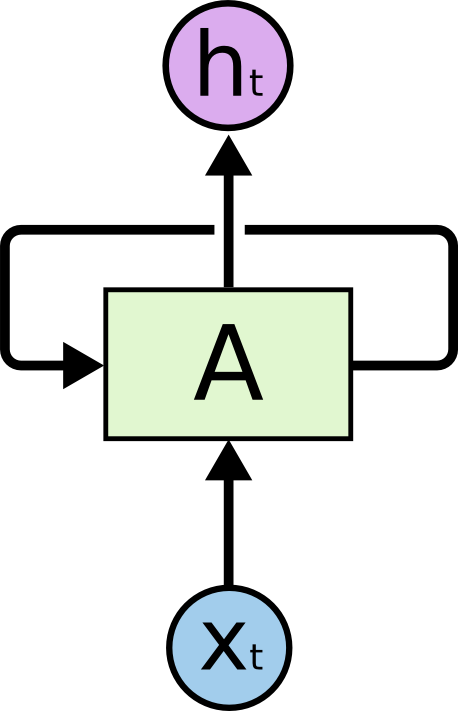
\includegraphics[scale=0.5]{RNN-rolled}
\caption{Recurrent Neural Network \protect\footnotemark}
\label{fig:rnn_rolled}
\end{figure}
\footnotetext{\url{https://colah.github.io/posts/2015-08-Understanding-LSTMs/}}

The sequential information is preserved in the hidden state of the RNN, which spans many time steps as it cascades forward to affect the processing of future inputs. This builds a correlation between temporal events that was impossible to do in MLPs. Since an event or input may depend on a far (in time) predecessor, these correlations are called ``long-term dependencies''. Mathematically this information cascade can be modeled as the recursive relation:
\[ \mathbf{h}_t = f (\mathbf{W}_x \cdot \mathbf{x}_t + \mathbf{W}_h \cdot \mathbf{h}_{t-1}) \]

where $\mathbf{W}_x, \mathbf{W}_h$ are weight matrices and $f$ is an activation function. That is to say; the hidden state at the current time step $\mathbf{h}_t$ is a function of the current input $\mathbf{x}_t$ and the hidden state at the previous time step $\mathbf{h}_{t-1}$.

RNNs are trained through an extension of backpropagation called backpropagation through time (BPTT) \citep{werbos1988generalization}. Time, in this context, is modeled as an ordered series of calculations linking one time step to the next, allowing backpropagation to work.


\subsection{Bidirectional Recurrent Neural Networks}
\label{sec:birnns}

One of the flaws of vanilla RNNs is that it suffers from the limitation of using input information just up to the present time step. In word classification applications that rely heavily on context (e.g., named entity recognition), vanilla RNNs fall short. The limitation restraints the RNN from learning any information about the future context. In fact, an easy solution was proposed \citep{schuster1997bidirectional} by stacking two RNNs, one working in the forward direction while the other works in the backward direction.

A Bidirectional RNN (Bi-RNN) is a composition of two RNNs, where the input sequence is fed normally to the first network and fed in reverse to the second one -- as shown in \cref{fig:bi_rnn}. At any time step $t$, the Bi-RNN would have learned two representations of the input text; $h_{t-1}$ the hidden representation of the past inputs up to input $x_t$, and $h'_{t-1}$ the hidden representation of the future inputs after the input $x_t$.

\begin{figure}[ht]
\centering
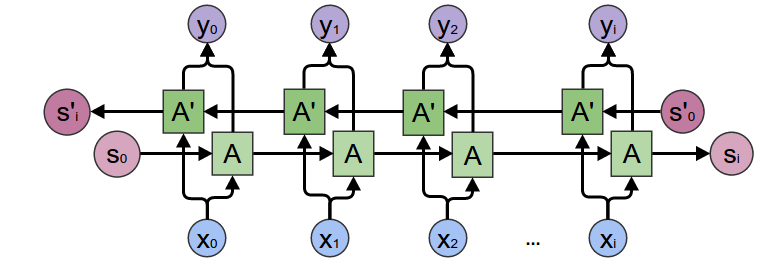
\includegraphics[scale=0.5]{RNN-bidirectional}
\caption{Bidirectional Recurrent Neural Network \protect\footnotemark}
\label{fig:bi_rnn}
\end{figure}
\footnotetext{\url{https://colah.github.io/posts/2015-09-NN-Types-FP/}}

Mathematically, the information propagation is modeled similarly to the RNN:
\[ \mathbf{h}_t = f (\mathbf{W}_x \cdot \mathbf{x}_t + \mathbf{W}_h \cdot \mathbf{h}_{t-1}) \]
\[ \mathbf{h}'_t = f' (\mathbf{W}'_x \cdot \mathbf{x}_t + \mathbf{W}'_h \cdot \mathbf{h}'_{t-1}) \]

Bi-RNNs are trained similarly to RNNs since the two stacked networks are independent of each other. However, applying BP to Bi-RNNs is exceedingly slow due to the very long dependency chain.

\subsection{Long Short-Term Memory Networks}
\label{sec:lstms}

A fundamental problem for vanilla RNNs is vanishing or exploding gradients. As RNNs became deeper to process longer sequences, the successive multiplication of the gradients through the many layers leads to the gradients becoming exceedingly small or large, thus making the learning process unstable. Exploding gradients can be easily handled through clipping or squashing.

Vanishing gradients, however, can cause a network to stop learning by not updating the weights. Long Short-Term Memory (LSTM) networks \citep{hochreiter1997long} were designed specifically to solve this problem. The LSTM unit replaces the standard RNN memory cell to preserve and control the gradient flow during backpropagation.

An LSTM unit as shown in \cref{fig:lstm_cell} consists of a cell and a gating system that controls the information flow through the cell. This control is based on the information's magnitude and importance, through a filtering system that is adjusted through the training process. This filtering system is composed of three gates; forget gate, input gate, and output gate.

\begin{figure}[ht]
\centering
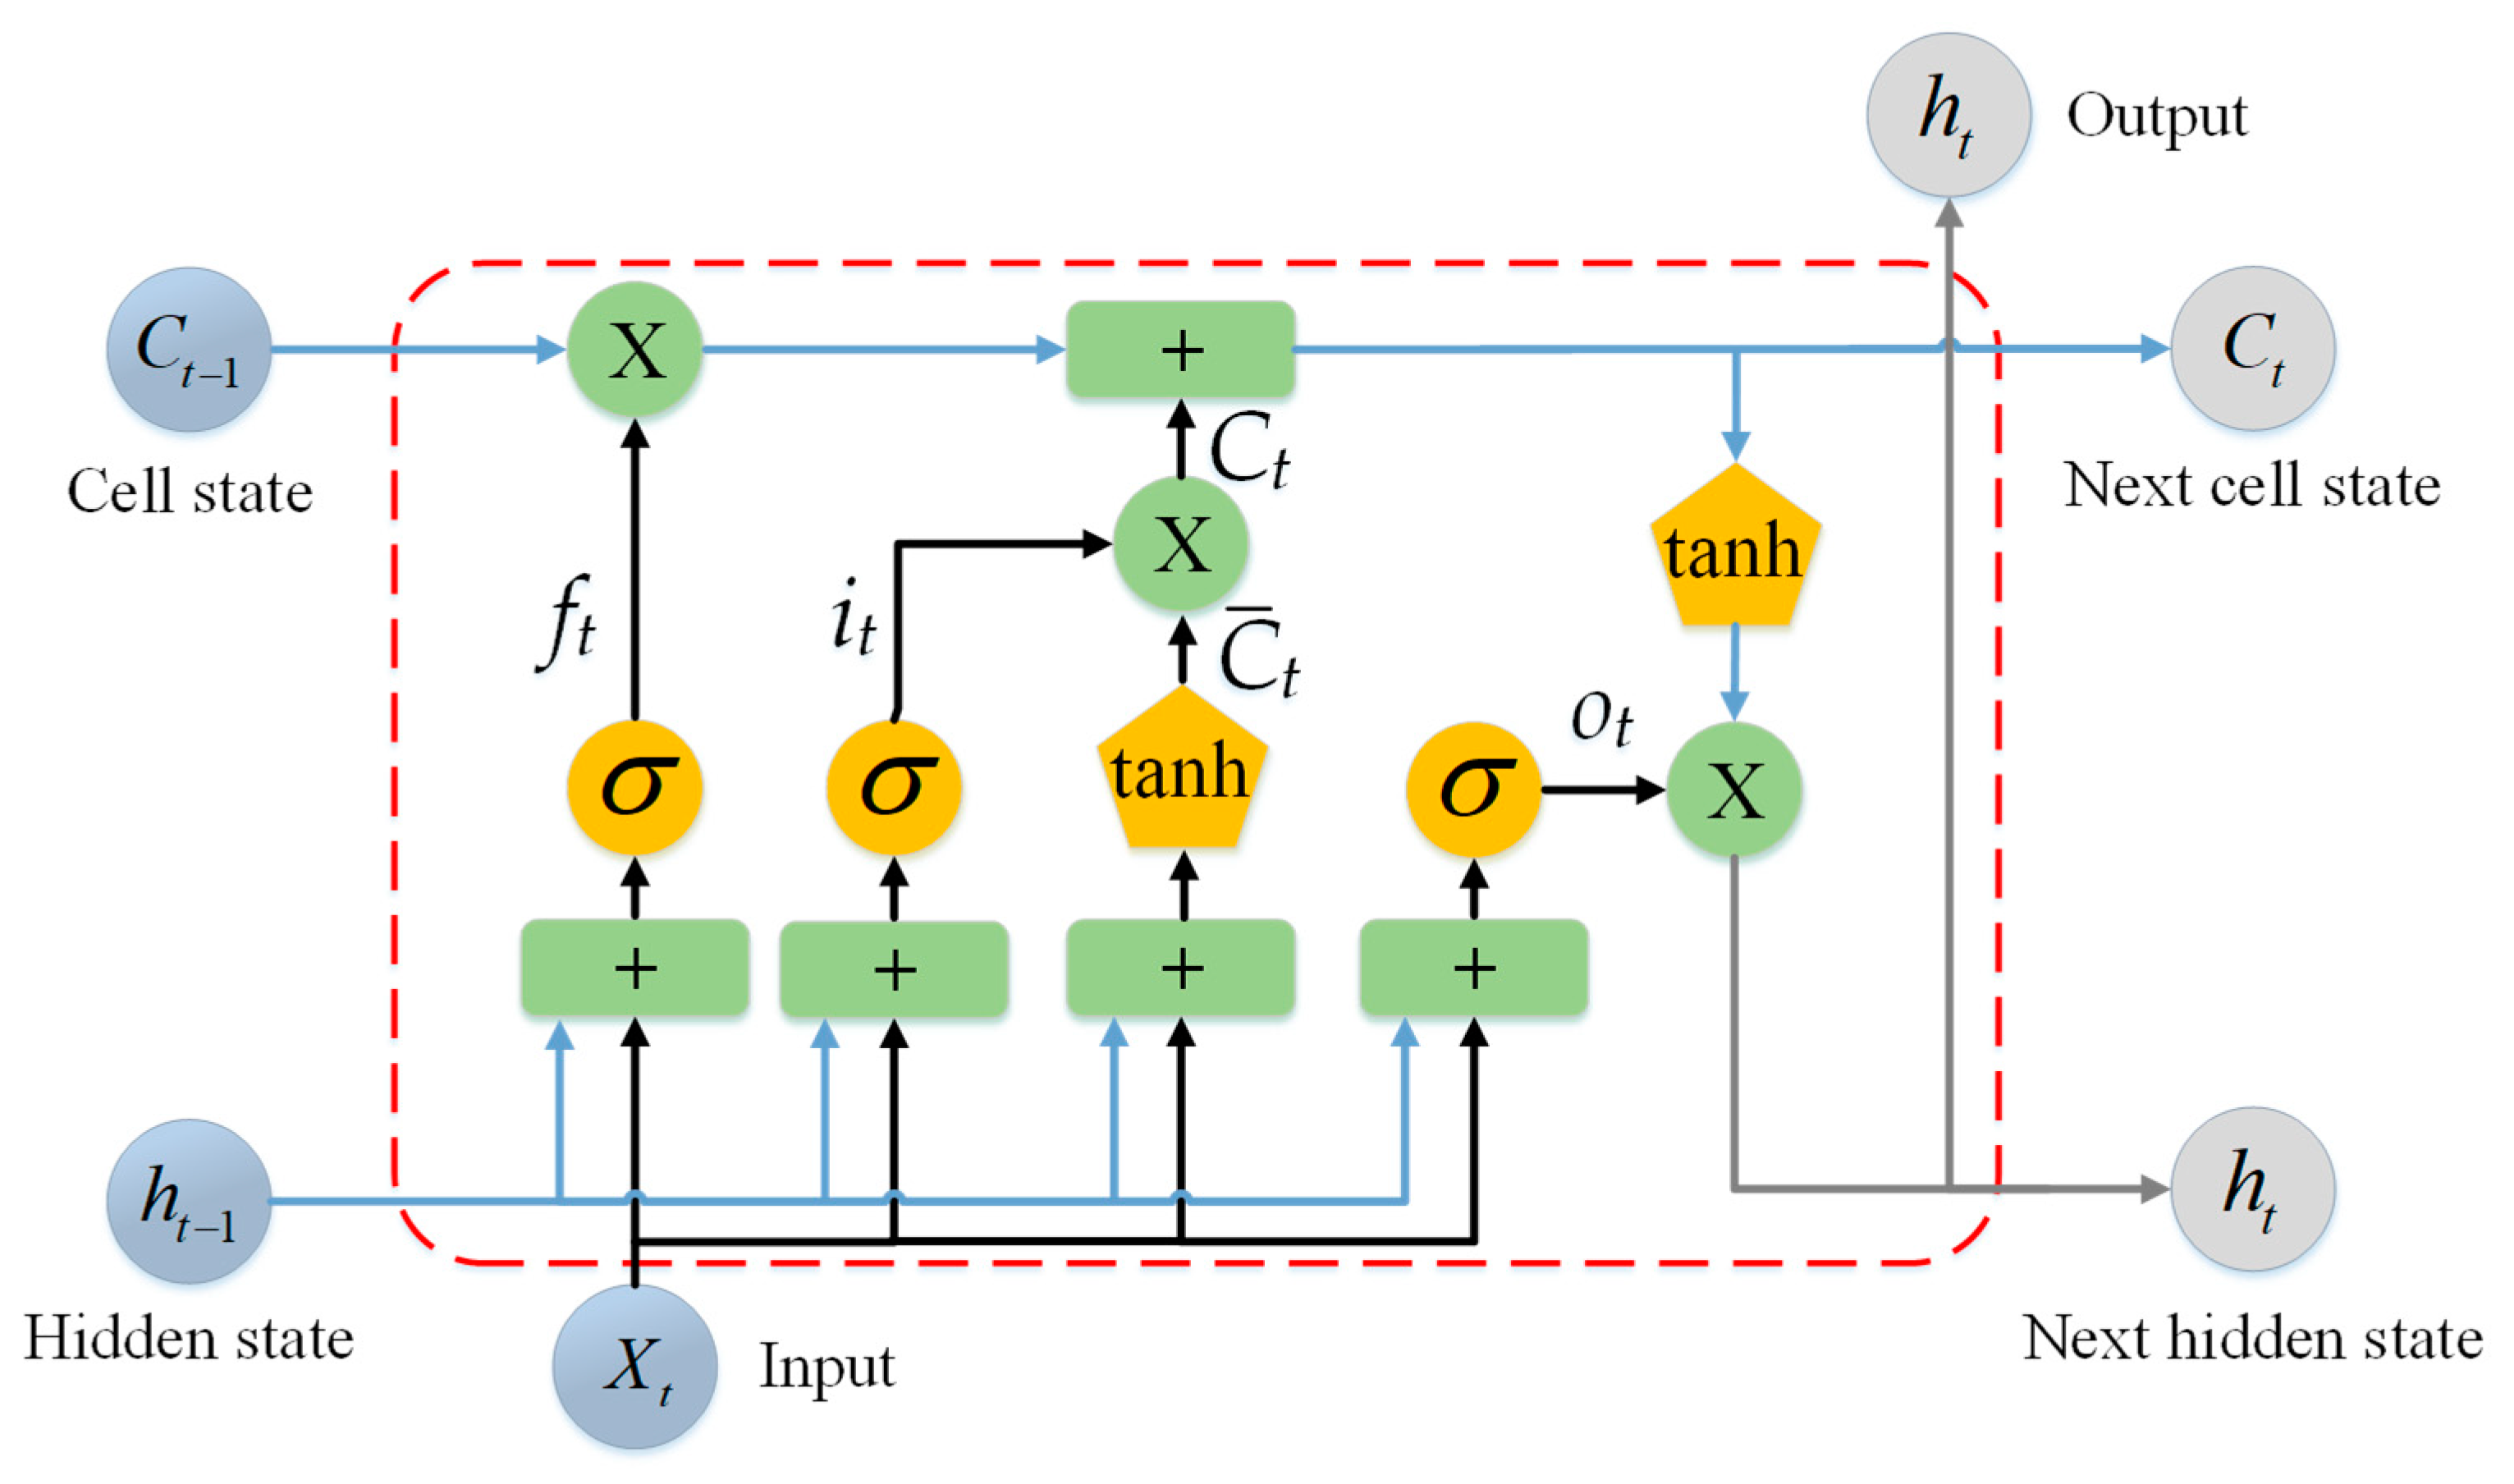
\includegraphics[scale=0.1]{LSTM-cell}
\caption{LSTM Unit \protect\footnotemark}
\label{fig:lstm_cell}
\end{figure}
\footnotetext{\url{https://www.mdpi.com/2079-9292/10/9/1026}}

The core idea behind LSTMs is manipulating the cell state by having the ability to remove, retain or add information to the cell state, regulated by the three gates. Gates learn to optionally let information through. They are composed of a sigmoid layer and a pointwise multiplication operation. The sigmoid output produces a weight [0, 1] of how much information should flow through the gate.

The forget gate decides what information is going to be removed from the cell state. It observes $h_{t-1}$ and $x_t$, and outputs a weight for every value in $C_{t-1}$. This mechanism is useful when the context changes for example. If our subject changes from one sentence to another, we want the LSTM to forget about the old subject and pay attention to the new one. The forget gate learns the following function:
\[ f_t = \sigma (\mathbf{W}_f \cdot [h_{t-1}, x_t] + b_f) \]

In order to register new information, the input gate is used to update the cell state. This is a two step process, first, we decide which values to update. Then, we create a candidate vector $\tilde{C}_t$ that would replace some elements in the cell state.
\[ i_t = \sigma(\mathbf{W}_i \cdot [h_{t-1}, x_t] + b_i) \]
\[ \tilde{C}_t = \tanh ( \mathbf{W}_C \cdot [h_{t-1}, x_t] + b_C ) \]

Next, we perform the cell update. Intuitively, the equation to update the cell state is:
\[ C_t = f_t * C_{t-1} + i_t * \tilde{C}_t \]

Finally, the output gate decides which pieces of the cell state to filter out and which to pass through as the output of the LSTM unit. We squish the cells state with a \texttt{tanh} activation and multiply it by the learned output gate to obtain the new hidden state $h_t$.
\[ o_t = \sigma (\mathbf{W}_o \cdot [h_{t-1}, x_t] + b_o) \]
\[ h_t = o_t * \tanh (C_t) \]

Training an LSTM network means repeatedly adjusting the weights for each gate to learn the optimal behavior to solve a specific task. A popular variant of the LSTM is the Gated Recurrent Unit (GRU). The GRU combines the forget and input gates into a single update gate, and it merges the cell state and the hidden state. The resulting model is much simpler and faster to train without much compromise on  performance.

It is worth noting that while feedforward networks map one input to one output, recurrent structures support a variety of mappings; one-to-many, many-to-one, and many-to-many.


% =================================================================================================

\section{Sequence-to-Sequence Architectures}
\label{sec:seq2seq}

Many applications in NLP are in the form of sequence transformations, that is transforming the input sequence to an output sequence (e.g. machine translation, text summarization, conversational agents), where both sequences can be of arbitrary length. A Sequence-to-Sequence architecture (Seq2Seq) as shown in \cref{fig:seq2seq} consists, mainly, of two networks; an encoder network and a decoder network. In the context of NLP, these networks are typically RNNs or a variant (\cref{sec:rnns}).

The seq2seq model works, first, by scanning the input sequence, token-by-token, with the encoder network. The encoder network is used to ``understand'' the input sequence and learns an associated fixed-size vector representation (context vector) of the whole sequence. The decoder network is initialized with this context vector and proceeds to generate an output sequence, in a token-by-token manner. This decoupling of reading and generation works well in practice on a variety of problems.

Seq2seq models were first introduced \citep{sutskever2014sequence} in the context of machine translation. This new LSTM based model was able to achieve state-of-the-art (SOTA) performance, without the need for any manual feature engineering. The advantage of seq2seq models is the ability to train them end-to-end, assuming the availability of parallel corpora.

\begin{figure}[ht]
\centering
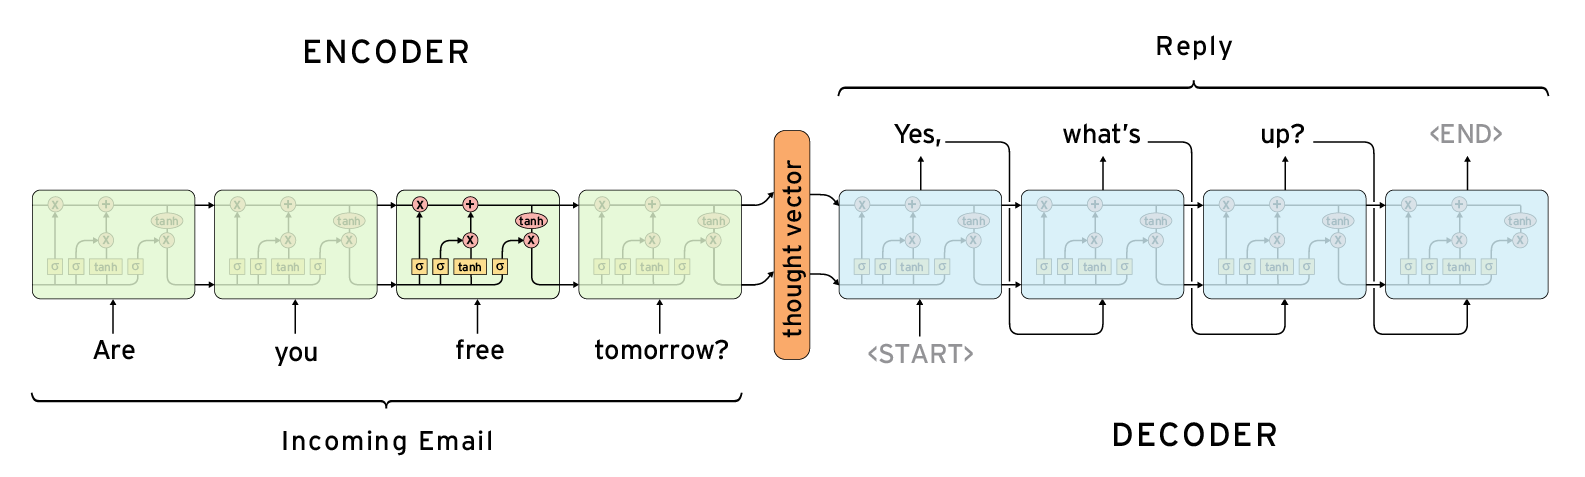
\includegraphics[scale=0.5]{seq2seq}
\caption{Encoder-Decoder Architecture \protect\footnotemark}
\label{fig:seq2seq}
\end{figure}
\footnotetext{\url{https://suriyadeepan.github.io/2016-12-31-practical-seq2seq/}}

The encoder network of the model is of autoencoding property, where it is trained to build a vector representation, of the whole input sequence, that should enable the network to reconstruct the input. In other words, the goal is to learn an efficient encoding that stores the right pieces of information required for reconstruction. Recently, models have been proposed that use the encoder part only of the architecture. Encoders are usually used for language understanding tasks, such as sentence classification or token classification.

The decoder network of the model is of autoregressive property, where it is trained to generate outputs depending on the previous inputs and the hidden state. The decoder defines a probability over the output $\mathbf{y}$ by decomposing the joint probability into conditional probabilities:
\[ p(\mathbf{y}) = \prod_{t=1}^{T_y}  p(y_t \mid \{y_1, \ldots, y_{t-1}\}, \mathbf{c}) \]
with $\mathbf{c}$ being the context vector learned by the encoder.

Similarly, networks with decoder-only components have been in use. Decoders are usually used for language generation tasks, such as text summarization or dialog systems (chatbots).


% =================================================================================================

\section{Attention Mechanism}
\label{sec:attention}

Although seq2seq models work well in practice, the attempt to compress the whole input sequence in a fixed-size context vector is very limiting and sometimes a difficult task. The encoder is very likely to forget some relevant information in longer input sequences. Also, the decoder may need to ``focus'' more on different parts of the input while generating the output at different time steps.

The attention mechanism was first proposed \citep{bahdanau2014neural} to help memorize longer source sentences in neural machine translation. The main concept behind attention is to enable the decoder to have a direct view of the source sequence via the entire sequence of encoder hidden states. These shortcut connections (between the encoder and the decoder) are learnable for each output time step.

Even though the context vector has access to the entire input sequence, its function is now different. Instead of trying to compress the input, it now controls the alignment between the source and target. This alignment is conditioned on: (1) encoder hidden states, (2) decoder hidden states, and (3) alignment weights which represent how well input and output tokens match.

The context vector is computed as a weighted sum of the encoder hidden states:
\[ c_i = \sum_{j=1}^{T_x} \alpha_{ij} h_j \]

The alignment weights $\alpha_{ij}$ are computed by:
\[ \alpha_{ij} = \frac{\exp(e_{ij})}{\sum_{k=1}^{T_x} \exp(e_{ik})}\, , \quad e_{ij} = a(s_{i-1}, h_j) \]
where $e_{ij}$ is parameterized as a feedforward network conditioned on $s_{i-1}$ -- the decoder hidden state and $h_j$ -- the encoder hidden state. This network is trained jointly with other seq2seq components to learn the optimal alignment between target words and source words.

A variety of attention mechanisms have since been studied. We focus on a family of attention mechanisms called self-attention.


\subsection{Self-Attention}
\label{sec:self_attn}

Self-attention \citep{vaswani2017attention} is an attention mechanism that relates different positions of the same sequence to compute a contextual representation of that sequence. The scores of self-attention are computed in parallel which results in an order of magnitude improvement over RNNs, which need to process data sequentially. 

To calculate the self-attention model, we create three distinct representations of the sequence $\mathbf{X}$; $\mathbf{Q} = \mathbf{X} \mathbf{W}_Q$ -- query, $\mathbf{K} = \mathbf{X} \mathbf{W}_K$ -- key, and $\mathbf{V} = \mathbf{X} \mathbf{W}_V$ -- value, with $\mathbf{W}_Q, \mathbf{W}_K, \mathbf{W}_V$ learnable weight matrices. This query-key-value concept is borrowed from information retrieval systems. When you search for a \textit{query}, the search engine will map the query against a set of \textit{keys} associated with possible results. Then an algorithm will return the best-matching results (\textit{values}).

This process in information retrieval literature is called content-based lookup \citep{mitra2000information}, hence the name \textit{content-based} self-attention. In the self-attention mechanism, this idea of retrieving an object is relaxed. We define a degree of similarity between our representations to be able to weigh our query. Instead of choosing where to look depending on the position in the sequence, we can attend to the content we need itself. That is why we need to separate keys from values; the keys are used to calculate the attention weights while the values define the information we \textit{retrieve}.

We can now define the self-attention mechanism mathematically:
\[ \text{Self-Attention}(\mathbf{Q}, \mathbf{K}, \mathbf{V}) = \text{softmax} \Big(\frac{\mathbf{Q} \mathbf{K}^T}{\sqrt{d_k}}\Big) \mathbf{V} \]
where we notice the similarity measure using a scaled dot-product. The scaling is to prevent the problem of exploding gradients. The \texttt{softmax} activation is used to get the final attention weights as a probability distribution.


\subsection{Multi-Head Self-Attention}
\label{sec:multihead_attn}

Multi-Head Self-Attention \citep{vaswani2017attention} can be thought of, simply, as an ensemble of independent self-attention mechanisms running also in parallel. In this context, the output of a single self-attention model is called a ``head'', the outputs of different heads are concatenated and linearly transformed into the expected dimension (see \cref{fig:multi_head_attn}). This composition of heads allows the model to jointly learn different representations of the input which improves the final attention-based representation.
\[ \text{Multi-Head} (\mathbf{Q}, \mathbf{K}, \mathbf{V}) = [\text{head}_1; \ldots; \text{head}_n] \mathbf{W}_O \]
where each head is the output of the scaled dot-product attention (\cref{sec:self_attn}).

\begin{figure}[ht]
\centering
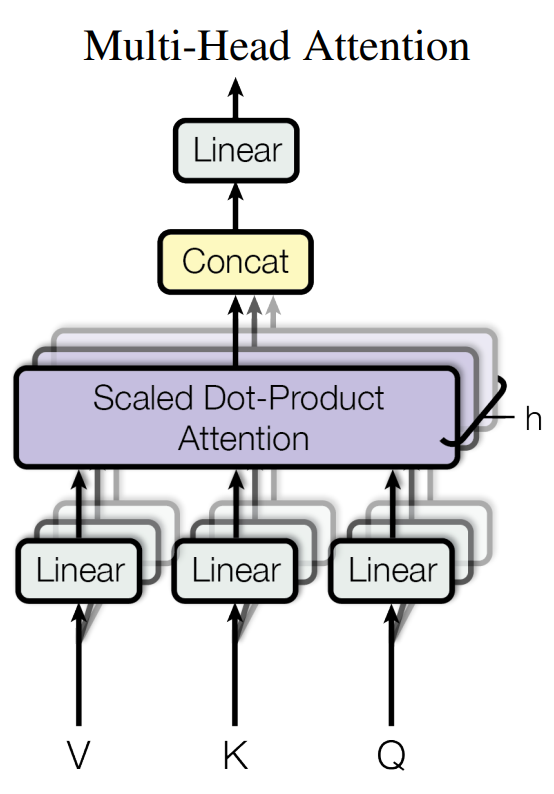
\includegraphics[scale=0.3]{multi_head_attn}
\caption{Multi-Head Self-Attention \protect\footnotemark}
\label{fig:multi_head_attn}
\end{figure}
\footnotetext{Attention is all you need. \citep{vaswani2017attention}}


% =================================================================================================

\section{Transformers}
\label{sec:transformers}

Recurrent architectures process input data sequentially to build a vector representation that is used in downstream tasks. Several models have been proposed to improve this limitation and have sequential data processed in parallel. ByteNet \citep{kalchbrenner2016neural} and ConvS2S \citep{gehring2017convolutional} use convolutional neural networks (CNNs) as basic building block to compute hidden representations in parallel for input and output positions. In these models, the number of calculations required to relate two arbitrary input and output positions grows in the distance between positions, linearly for ConvS2S and logarithmically for ByteNet. This makes it more expensive to learn representations for longer sequences.

The Transformer architecture was introduced \citep{vaswani2017attention} to solve this problem. Transformers are entirely built on the multi-head self-attention mechanism, without any recurrent units. The number of required calculations required to relate two arbitrary positions is now constant.

The Transformer is an encoder-decoder architecture -- shown in \cref{fig:transformer} -- based on multi-head self-attention modules and normalization layers with residual skip connections.

An encoder block consists of: (1) multi-head self-attention layers (discussed in \cref{sec:multihead_attn}), (2) feedforward layers applied on the attention layer output to project it in a higher-dimensional space, (3) residual skip connections which are shortcut connections to add the input of the sub-layer to its output; this was found to improve gradient flow while adding more layers, and finally, (4) layer normalization \citep{ba2016layer} which independently normalizes the vector representation for each token -- this improves convergence stability.

A decoder block is similar to an encoder block with exceptions. The first multi-head attention is modified to mask the latter positions to prevent the decoder from attending to subsequent positions during predicting the current token. The second multi-head attention takes input from both the previous sub-layer and the encoder.

\begin{figure}[ht]
\centering
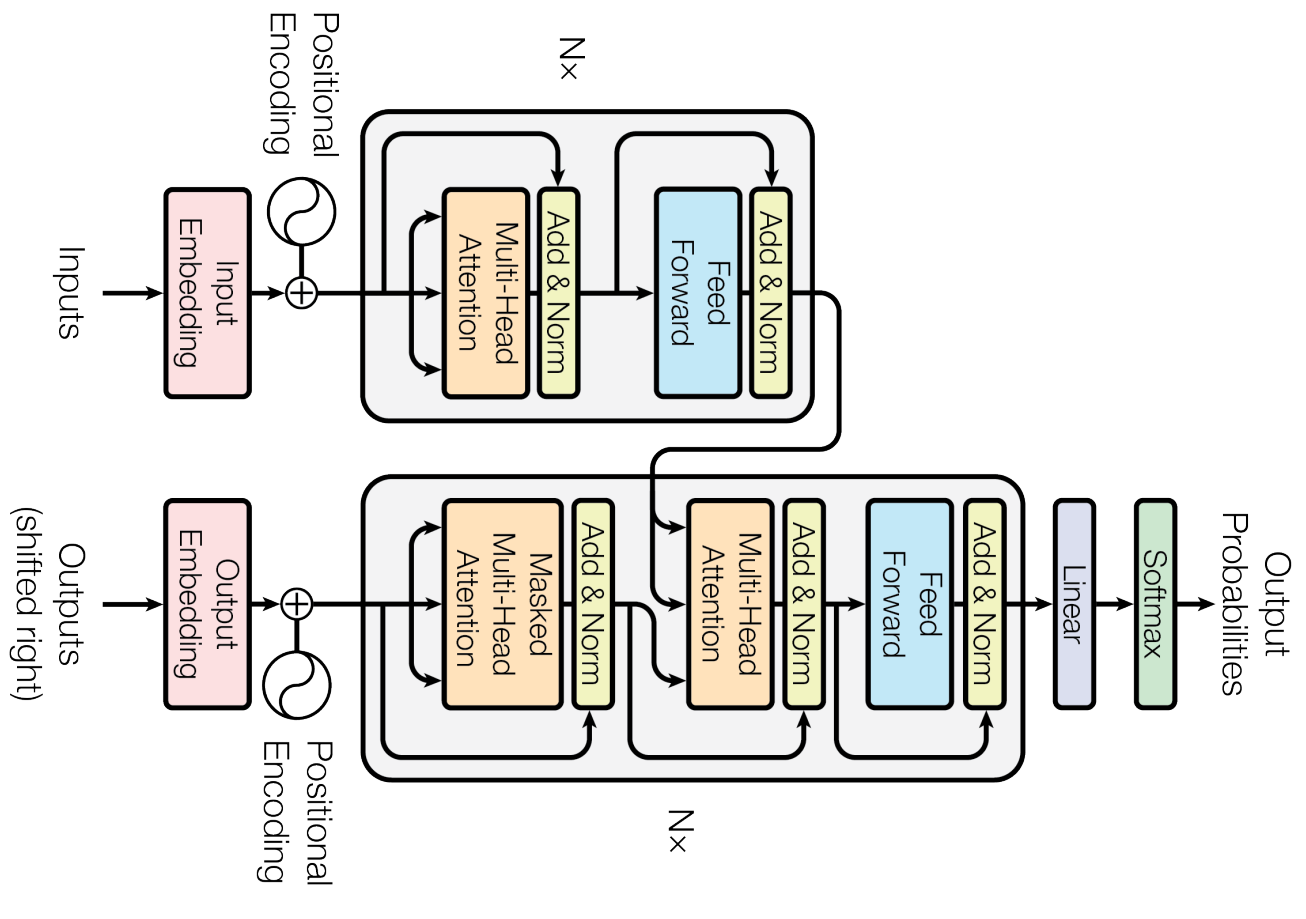
\includegraphics[scale=0.3, angle=90]{transformer}
\caption{Full Architecture of the Transformer. Encoder (left) and Decoder (right). \protect\footnotemark}
\label{fig:transformer}
\end{figure}
\footnotetext{Attention is all you need. \citep{vaswani2017attention}}

\subsection{Positional Embeddings}
\label{sec:pos_embeddings}

All word embedding techniques (\cref{sec:embeddings}) incorporate information about the token's position in some way -- a context window, a recurrence, or a convolution. However, in Transformers we completely remove the sequential processing mechanism of the RNN in favor of the parallelism of self-attention. In turn, this led to the loss of positional information for input tokens.

The authors of the original Transformer paper \citep{vaswani2017attention} introduced a function $f \colon \mathbb{N} \mapsto \mathbb{R}^d$ to compute the positional encoding $p_t$ for a token at position $t$ as follows:
\[
p_t^{(i)} = f(t) ^ {(i)} = \begin{cases}
	\sin(\omega_k \cdot t), & \text{ if } i = 2k \\
	\cos(\omega_k \cdot t), & \text{ if } i = 2k + 1\\
\end{cases}
\]
where $\omega_k = \dfrac{1}{10000^{2k/d}}$ and $i$ is the dimension. This output vector $p_t$ is then added to the input embeddings -- where they have the same size.

This type of embeddings was chosen since: (1) it is unique and deterministic for each token, (2) allows the model to generalize to longer sequences than those encountered in training, and (3) allows the model to attend by relative positions efficiently.

Finally, thanks to the use of residual skip connections through the Transformer blocks, the positional information is efficiently propagated to higher-level layers where more complex interactions are handled.


\subsection{Pretrained Transformer Models}
\label{sec:pretrained_models}

The ability to train models quickly through enhanced hardware capabilities combined with improved learning algorithms has led to a paradigm shift in deep learning. In NLP, this shift came with the rise of transformers which could be trained faster, by order of magnitudes, than recurrent architectures and on longer sequences with better results.

Transfer Learning is a method of reusing the information (weights) learned by one trained model, on some task, in another model that is required to perform a different but related, task \citep{Goodfellow-et-al-2016}. This is done by using \textit{pretrained} models in some way. One can either continue training those learned weights on the required task (fine-tuning) or simply freeze the weights and train only the output layer.

Transfer learning opened the window for accessible state-of-the-art models to be used in all scenarios without the difficult requirements of obtaining such models.

\subsubsection{BERT}
\label{sec:bert_intro}

One of the most famous pretrained transformer models is BERT which was developed by Google. BERT \citep{devlin2018bert} -- or Bidirectional Encoder Representations from Transformers -- outperformed other NLP models when it was released in many language-related tasks. It builds on top many clever ideas that were proposed by several researchers, like semi-supervised sequence learning \citep{dai2015semi}, ELMo \citep{peters2018deep}, ULMFiT \citep{howard2018universal}, and the Transformer \citep{vaswani2017attention} among others.

BERT uses encoder blocks from the vanilla transformer and is most suitable for language understanding tasks (e.g., sequence classification, next token prediction). The first innovative addition in BERT is that it uses a bidirectional self-attention mechanism in contrast to left-to-right self-attention used in the vanilla transformer. This idea leads to an improved contextual representation for tokens. However, it also creates a problem where each word would be able to attend to itself in a multi-layered context, thus leading to corrupted training.

To solve this problem, the authors propose to randomly mask some of the input tokens and have the model learn how to reconstruct these tokens based on the context. This task is called Masked Language Modeling (MLM). The mask's value can be a generic value or sometimes a word is replaced with another to improve fine-tuning on downstream tasks.

Another pretraining task used is Next Sentence Prediction (NSP). Many downstream tasks require the understanding of the relationship between two sentences (e.g., Question Answering, Natural Language Inference). This task is cast to a binary classification task where BERT simply decides whether the latter sentence follows the first.

After pretraining BERT on the two previously mentioned tasks, it can be fine-tuned to solve a variety of language understanding problems. One other way to use BERT is as a feature extractor, where BERT is used to produce contextual word embeddings which are then fed to any model of choice on some related task.

\subsubsection{BART}
\label{sec:bart_intro}

BERT-like models perform well where the prediction at position $i$ is allowed to use information from later positions. This is, however, not practical in text generation tasks, where the prediction for position $i$ can depend only on previous positions. On the other hand, autoregressive models, such as GPT \citep{radford2018improving}, are pretrained to predict the next word while masking future positions making it more suitable for generation tasks. It follows that GPT-like models are unable to generalize well on downstream tasks where the whole input contributes information for the output.

BART \citep{lewis2019bart} combines the best of both approaches. It utilizes the full transformer architecture, with a BERT bidirectional encoder and a GPT autoregressive decoder, along with a variety of pretraining tasks. BART is pretrained on (1) token masking similar to BERT, (2) token deletion, where random tokens are deleted and the model must predict their correct positions, (3) text infilling, where a span of text (sequence of tokens) is masked by a single mask and the model must predict how many tokens were masked, (4) sentence permutation, where sentences of a document are shuffled in random order, and finally, (5) document rotation, where a document is rotated to start from a given token and the model is asked to predict the correct starting token.

BART performs best when fine-tuned on text generation tasks, but also works well for language comprehension tasks.

